\section{Pointers and references}

\subsection{Overview of pointers and references}
\subsubsection*{References}
Note that references are typically safer to use than pointers because they cannot
be reassigned.
\begin{itemize}
	\item Is an alias for something (i.e. another name for an already existing variable.
	\item Need to be initialised and cannot be reassigned.
	\item All performed on the reference variable also happens to the original.
	\item Declaration with the ampersand,\emph{\&} \ldots
\end{itemize}

\begin{minted}
[frame=lines, linenos, fontsize=\small, obeytabs=true, tabsize=3]{c++}
int& referance_v_as_alias_of = my_name;
\end{minted}

\begin{itemize}
	\item The double meaning of \emph{\&} \ldots
	\begin{itemize}
		\item In a declaration (i.e. at initialisation or as a function parameter) it is
		a reference parameter.
		\item Not in a declaration it is an address operator.
	\end{itemize}
\end{itemize}


\subsubsection*{Pointers}
\begin{itemize}
	\item Stores a memory address.
	\item Pointers are reassignable.
	\item Pointer has their own memory address while references do not (i.e. you
	can have a pointer to a pointer but not a reference of a reference).
	\item Declaration \ldots
\end{itemize}

\begin{minted}
[frame=lines, linenos, fontsize=\small, obeytabs=true, tabsize=3]{c++}
int* pointer_name = &some_variable;

//OR

int* pointer_name;
pointer_name = &some_variable;

//OR using a typedef
typedef int* int_pointer;
int_pointer a, b, c; //declares 3 pointer variables

\end{minted}

\subsubsection*{Overview of fetures of pointers, references, and const pointers}

\begin{table}[H]
\begin{center}
\renewcommand{\arraystretch}{1.8}
\begin{tabular}{ m{3cm} m{3cm} m{3cm} m{3cm}} 
\textbf{Concept} & \textbf{nullable} & \textbf{(re)assignable} &\textbf{arithmetic}\\
\hline
Pointer & yes & yes & yes\\
\hline
const Pointer & yes & no & yes\\
\hline
Reference & no & no & no\\
\hline
\end{tabular}
\end{center}
\caption{Overview of features of pointers, const pointers, and references}
\label{table_1}
\end{table}

Note (( think) that if you call a function with an \& next to the argument, then the declaration
of this function requires the corresponding parameter to have a \* (i.e. to be a pointer) \ldots{}
but check this again.

%---------------------------------------------
\subsection{Illustration of when to use a reference, const ref, pointer, or pass by value}

%Define block styles
\tikzstyle{bitwise} = [diamond, draw, fill=blue!20, 
text width=6em, text centered, node distance=3cm, inner sep=0pt]

\tikzstyle{decision_1} = [rectangle, draw, fill=blue!10, 
text width=9em, text centered, minimum height=4em]

\tikzstyle{decision_2} = [rectangle, draw, fill=yellow!20, 
text width=9em, text centered, minimum height=4em]

\tikzstyle{result} = [rectangle, draw, fill=green!20, 
text width=9em, text centered, minimum height=4em]

\tikzstyle{line} = [draw, -latex']
\tikzstyle{cloud} = [draw, ellipse,fill=red!20, node distance=3cm,
minimum height=4em]

\begin{figure}[H]
  \centering
  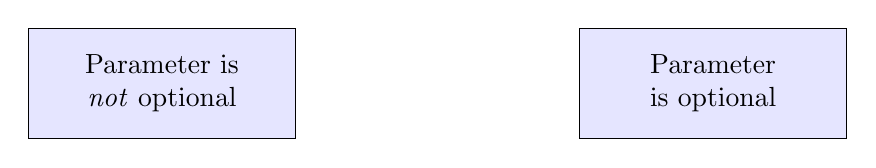
\begin{tikzpicture}[node distance = 2cm, auto]
	%decsision_2/.style={sibling distance=40mm},
	%edge from parent/.style={->,draw}, >=latex]
  	
	%Nodes
	\node [decision_1] (init) {Parameter is \emph{not} optional};
		
		%child {node [decision_2] (3) {Type is \emph{expensive} to copy}}
		
		%child {node [decision_2] (4) {Type is cheap to copy \emph{and} parameter is not modified}};

	\node [decision_1, right of = init, node distance = 7cm] (2) {Parameter is optional};
	
  	%Lines
	%\path [line] (assess) -- (nutrition);
  
  \end{tikzpicture}
\end{figure}


%---------------------------------------------
\subsection{Pointers}
\subsubsection*{The \emph{new} operatator}

\begin{itemize}
	\item Used to create dynamic variables (have no identifiers to serve as their
	variable names).
	\item Dynamic variables are stored on the heap.
	\item Refer to the values of these variables using dereferenced pointers.
\end{itemize}

\begin{minted}
[frame=lines, linenos, fontsize=\small, obeytabs=true, tabsize=3]{c++}
p1 = new int; //creates new dynamic variable (has no variable name)
cin >> *p1; // assign a number to the variable
*p1 = *p1 + 7; // add 7 to the variable
\end{minted}

\subsubsection*{The \emph{delete} operatator - return memory to the heap}
\begin{itemize}
	\item When deleting, the variable is then undefined - ensure to check if a pointer
	actually points to something before applying the dereferencing operator.
\end{itemize}

\begin{minted}
[frame=lines, linenos, fontsize=\small, obeytabs=true, tabsize=3]{c++}
// Make the following check before trying to assign a value to a dangling pointer
delete pointer;
pointer = NULL; //once it is NULL you cannot assign a value to the 
//dereferenced pointer

if (pointer != NULL){
    *pointer = 40;
} else {
    cout << "Dangling pointer";
    exit(1);
}
\end{minted}

\subsubsection*{Safety measure if there is not sufficient memory on heap to create a dynamic variable}
\begin{itemize}
	\item C++ would throw an exception called std::bad\_alloc.
	\item You can catch the error in two ways:
	\begin{enumerate}
		\item \emph{try \ldots catch} or
		\item Call to \emph{new (nowthrow)} and then set the corresponding pointer
		to NULL in case of allocation failure.
	\end{enumerate}
\end{itemize}

\noindent
1. Try catch
\begin{listing}[H]
\begin{minted}
[frame=lines, linenos, fontsize=\small, obeytabs=true, tabsize=3]{c++}
try
{
    ptr_a = new int;
}
catch
{
    cout << "Sorry, ran out of memory.";
    ptr_a = NULL;
    exit(1);
}
\end{minted}
\caption{Check that there is enough memory to create a dynamic pointer - v1}
\label{source_code}
\end{listing}

\noindent
2. Call to nothrow
\begin{listing}[H]
\begin{minted}
[frame=lines, linenos, fontsize=\small, obeytabs=true, tabsize=3]{c++}
ptr_a = new (nothrow) int;
if (ptr_a == NULL)
{
    cout << "Sorry ran out of memory."
}
\end{minted}
\caption{Check that there is enough memory to create a dynamic pointer - v2}
\label{source_code}
\end{listing}

But it would be more elegant to wrap this around a function (using a call by reference parameter).

\begin{minted}
[frame=lines, linenos, fontsize=\small, obeytabs=true, tabsize=3]{c++}
int main()
{
    char* c_pointer;
    assign_new_int(c_pointer);
}

// In function definition
void assign_new_int(char*& some_pointer)
{ // function parameter is a pointer that is called by reference?!
    some_pointer = new (nothrow) char;
    if (some_pointer == NULL)
    {
        cout << "Bad allocation."
        exit(1);
    }
}
\end{minted}


%---------------------------------------------
\subsection{Dynamic arrays}
Note that you can assign an array to a pointer variable (provided that they have the same
base type) - but the other way round is illegal.

\begin{minted}
[frame=lines, linenos, fontsize=\small, obeytabs=true, tabsize=3]{c++}
int a[10]; // declare array
int* pointer; // declare a pointer

pointer = a; // is legal

//BUT the following is NOT legal
a = pointer;
\end{minted}


\subsubsection*{Declare and delete a dynamic array}
\begin{minted}
[frame=lines, linenos, fontsize=\small, obeytabs=true, tabsize=3]{c++}
double* pointer;
pointer = new double[10];

// When deleting a dynamic array do NOT forget the '[]'
delete [] pointer;
\end{minted}

Can also use pointer arithmetic on arrays.

\begin{minted}
[frame=lines, linenos, fontsize=\small, obeytabs=true, tabsize=3]{c++}
int* d;

d = new int[10];

// The two below are equivalent:
d[5];
*(d+5);
\end{minted}


\subsubsection*{Summary on using a dynamic array}
\begin{itemize}
	\item Define a pointer type (optional): a type for a pointer to variables of the same
	type as the elements of the array (e.g. typedef double* double\_array\_pointer;).
	\item Declare a pointer variable: that will point to the dynamic array in memory
	and will serve as the name of the dynamic array (e.g. double\_array\_pointer a;)
	\item Call new: to create a dynamic array (e.g. a = new double[array\_size];)
	\item Use like ordinary array: Note that the pointer variable should not have any other
	pointer value assigned to it, but should be used like an array variable only (otherwise
	that may confuse the system).
	\item Call delete: When your program is finished with the dynamic variable, use \emph{delete}
	and empty [] along with the pointer variable to return memory to the heap (e.g. delete [] a;).
\end{itemize}

\begin{listing}[H]
\begin{minted}
[frame=lines, linenos, fontsize=\small, obeytabs=true, tabsize=3]{c++}
/* This program illustrates the use of dynamic arrays. It prompts
   the user for a list of integers, then outputs their average to
   the screen. */ 

#include <iostream>
#include <cstdlib>
using namespace std;

//Function to compute the average value of the integer 
//elements in an array "list[]" of length "length"
float average(int list[], int length);

int main()
{
	int no_of_integers, *number_ptr;
	
	cout << "Enter number of integers in the list: ";
	cin >> no_of_integers;
	
	number_ptr = new (nothrow) int[no_of_integers];
	if (number_ptr == NULL)
	{
		cout << "Sorry, ran out of memory.\n";
		exit(1);
	}
	
	cout << "type in " << no_of_integers; 
	cout << " integers separated by spaces:\n"; 
	for (int count = 0 ; count < no_of_integers ; count++)
		cin >> number_ptr[count];
	cout << "Average: " << average(number_ptr,no_of_integers) << "\n";
	
	delete [] number_ptr;
}

float average(int list[], int length)
{
	float total = 0;
	int count;
	for (count = 0 ; count < length ; count++)
		total += float(list[count]);
	return (total / length);
}
\end{minted}
\caption{Illustration of use of dynamic arrays}
\label{source_code}
\end{listing}





